
Many scripting languages include a function for zipping two sequences together. A typical zip operation will take two input sequences and return a pair of values for each position in both inputs: 

Consider the case of two sequences – they can be containers, iterators, or initialization lists:

\hspace*{\fill} \\ %插入空行
\begin{center}
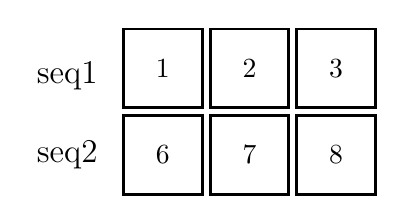
\begin{tikzpicture}
\foreach \x in {1,...,3} {
	\draw[line width=1pt] (1.1*\x,1) rectangle (1.1*\x+1,0) node[pos=.5] {\x};
}

\foreach \x [evaluate=\x as \index using int(\x+5)] in {1,...,3} {
	\draw[line width=1pt] (1.1*\x,-0.1) rectangle (1.1*\x+1,-1.1) node[pos=.5] {\index};
}

\node[text width=3cm, font=\large] at (1.5, 0.4) {seq1};
\node[text width=3cm, font=\large] at (1.5,-0.6) {seq2};
\end{tikzpicture}

Figure 4.6 – Containers to be zipped
\end{center}

We want to zip them together to make a new sequence with pairs of elements from the first two sequences:

\hspace*{\fill} \\ %插入空行
\begin{center}
\begin{tikzpicture}
\node[text width=3cm, font=\large] at (1.2, 0.4) {seq1};
\node[text width=3cm, font=\large] at (1.2,-0.6) {seq2};
\node[text width=3cm, font=\large] at (0.9,-2.5) {zipped};

\draw[line width=1pt] (1,1) rectangle (2,0) node[pos=.5] {1};
\draw[line width=1pt] (3.5,1) rectangle (4.5,0) node[pos=.5] {2};
\draw[line width=1pt] (6,1) rectangle (7,0) node[pos=.5] {3};

\draw[line width=1pt] (2.1,-0.2) rectangle (3.1,-1.2) node[pos=.5] {6};
\draw[line width=1pt] (4.6,-0.2) rectangle (5.6,-1.2) node[pos=.5] {7};
\draw[line width=1pt] (7.1,-0.2) rectangle (8.1,-1.2) node[pos=.5] {8};

\draw[line width=1pt] (1,-3.0) rectangle (2,-2.0) node[pos=.5] {1};
\draw[line width=1pt] (2.1,-3.0) rectangle (3.1,-2.0) node[pos=.5] {6};

\draw[line width=1pt] (3.5,-3.0) rectangle (4.5,-2.0) node[pos=.5] {2};
\draw[line width=1pt] (4.6,-3.0) rectangle (5.6,-2.0) node[pos=.5] {7};

\draw[line width=1pt] (6,-3.0) rectangle (7,-2.0) node[pos=.5] {3};
\draw[line width=1pt] (7.1,-3.0) rectangle (8.1,-2.0) node[pos=.5] {8};


\draw[decorate,decoration={calligraphic brace,amplitude=2mm, mirror},ultra thick] (1.5,-3.2) -- (2.6,-3.2);
\draw[decorate,decoration={calligraphic brace,amplitude=2mm, mirror},ultra thick] (4,-3.2) -- (5.1,-3.2);
\draw[decorate,decoration={calligraphic brace,amplitude=2mm, mirror},ultra thick] (6.5,-3.2) -- (7.6,-3.2);

\draw[line width=2pt][-latex] (1.5,-0.1) -- (1.5,-1.9);
\draw[line width=2pt][-latex] (2.6,-1.3) -- (2.6,-1.9);

\draw[line width=2pt][-latex] (4,-0.1) -- (4,-1.9);
\draw[line width=2pt][-latex] (5.1,-1.3) -- (5.1,-1.9);

\draw[line width=2pt][-latex] (6.5,-0.1) -- (6.5,-1.9);
\draw[line width=2pt][-latex] (7.6,-1.3) -- (7.6,-1.9);

\node[text width=3cm, font=\large] at (3.2,-3.7) {pair};
\node[text width=3cm, font=\large] at (5.7,-3.7) {pair};
\node[text width=3cm, font=\large] at (8.2,-3.7) {pair};
\end{tikzpicture}

Figure 4.7 – Zip operation
\end{center}

In this recipe we will accomplish this task with an iterator adapter.

\subsubsection{How to do it…}

In this recipe we'll build a zip iterator adapter that takes two containers of the same type  and zips the values into std::pair objects:

\begin{itemize}
\item 
In our main() function we want to call our adapter with two vectors:

\begin{lstlisting}[style=styleCXX]
int main()
{
	vector<std::string> vec_a {"Bob", "John", "Joni"};
	vector<std::string> vec_b {"Dylan", "Williams",
		"Mitchell"};
	cout << "zipped: ";
	for(auto [a, b] : zip_iterator(vec_a, vec_b)) {
		cout << format("[{}, {}] ", a, b);
	}
	cout << '\n';
}
\end{lstlisting}

This allows us to use the zip\_iterator in place of the individual vector iterators.

And we expect an output like this:

\begin{tcblisting}{commandshell={}}
zipped: [Bob, Dylan] [John, Williams] [Joni, Mitchell]
\end{tcblisting}

\item 
Our iterator adapter is in a class called zip\_iterator. We'll start with some type aliases for convenience:

\begin{lstlisting}[style=styleCXX]
template<typename T>
class zip_iterator {
	using val_t = typename T::value_type;
	using ret_t = std::pair<val_t, val_t>;
	using it_t = typename T::iterator;
\end{lstlisting}

These allow us to conveniently define objects and functions.

\item 
We don't store any data in our iterator. We only store copies of the target containers' begin() and end() iterators:

\begin{lstlisting}[style=styleCXX]
it_t ita_{};
it_t itb_{};
// for begin() and end() objects
it_t ita_begin_{};
it_t itb_begin_{};
it_t ita_end_{};
it_t itb_end_{};
\end{lstlisting}

ita\_ and itb\_ are iterators from the target containers. The other four iterators are used to generate the begin() and end() iterators for the zip\_iterator adapter.

\item 
We also have a private constructor:

\begin{lstlisting}[style=styleCXX]
// private constructor for begin() and end() objects
zip_iterator(it_t ita, it_t itb) : ita_{ita}, itb_{itb}
{}
\end{lstlisting}

This is used later to construct adapter objects specifically for begin() and end() iterators.

\item 
In the public section, we start with the iterator traits type definitions:

\begin{lstlisting}[style=styleCXX]
public:
using iterator_concept =
	std::forward_iterator_tag;
using iterator_category =
	std::forward_iterator_tag;
using value_type = std::pair<val_t, val_t>;
using difference_type = long int;
using pointer = const val_t*;
using reference = const val_t&;
\end{lstlisting}

\item 
The constructor sets up all the private iterator variables:

\begin{lstlisting}[style=styleCXX]
zip_iterator(T& a, T& b) :
	ita_{a.begin()},
	itb_{b.begin()},
	ita_begin_{ita_},
	itb_begin_{itb_},
	ita_end_{a.end()},
	itb_end_{b.end()}
{}
\end{lstlisting}

\item 
We define the minimum operator overloads to work with a forward iterator:

\begin{lstlisting}[style=styleCXX]
zip_iterator& operator++() {
	++ita_;
	++itb_;
	return *this;
}
bool operator==(const zip_iterator& o) const {
	return ita_ == o.ita_ || itb_ == o.itb_;
}
bool operator!=(const zip_iterator& o) const {
	return !operator==(o);
}
ret_t operator*() const {
	return { *ita_, *itb_ };
}
\end{lstlisting}

\item 
And finally, the begin() and end() functions return the respective iterators:

\begin{lstlisting}[style=styleCXX]
zip_iterator begin() const
	{ return zip_iterator(ita_begin_, itb_begin_); }
zip_iterator end() const
	{ return zip_iterator(ita_end_, itb_end_); }
\end{lstlisting}

These are made simple by the stored iterators and the private constructor.

\item 
Now let's expand our main() function for testing:

\begin{lstlisting}[style=styleCXX]
int main()
{
	vector<std::string> vec_a {"Bob", "John", "Joni"};
	vector<std::string> vec_b {"Dylan", "Williams",
		"Mitchell"};
	
	cout << "vec_a: ";
	for(auto e : vec_a) cout << format("{} ", e);
	cout << '\n';
	
	cout << "vec_b: ";
	for(auto e : vec_b) cout << format("{} ", e);
	cout << '\n';
	
	cout << "zipped: ";
	for(auto [a, b] : zip_iterator(vec_a, vec_b)) {
		cout << format("[{}, {}] ", a, b);
	}
	cout << '\n';
}
\end{lstlisting}


\item 
This gives us the output we're looking for:

\begin{tcblisting}{commandshell={}}
vec_a: Bob John Joni
vec_b: Dylan Williams Mitchell
zipped: [Bob, Dylan] [John, Williams] [Joni, Mitchell]
\end{tcblisting}

\end{itemize}

\subsubsection{How it works…}

The zipped iterator adapter is an example of how flexible the iterator abstraction can be.
We can take the iterators of two containers and use them in one aggregated iterator. Let's see how this works.

The main constructor for the zip\_iterator class takes two container objects. For the purposes of this discussion, we'll refer to these objects as the target objects.

\begin{lstlisting}[style=styleCXX]
zip_iterator(T& a, T& b) :
	ita_{a.begin()},
	itb_{b.begin()},
	ita_begin_{ita_},
	itb_begin_{itb_},
	ita_end_{a.end()},
	itb_end_{b.end()}
{}
\end{lstlisting}

The constructor initializes the ita\_ and itb\_ variables from the target begin() iterators. These will be used to navigate the target objects. The target begin() and end() iterators are also saved for later use.

These variables are defined in the private section:

\begin{lstlisting}[style=styleCXX]
it_t ita_{};
it_t itb_{};
// for begin() and end() objects
it_t ita_begin_{};
it_t itb_begin_{};
it_t ita_end_{};
it_t itb_end_{};
\end{lstlisting}

The it\_t type is defined as the type of the target iterator class:

\begin{lstlisting}[style=styleCXX]
using val_t = typename T::value_type;
using ret_t = std::pair<val_t, val_t>;
using it_t = typename T::iterator;
\end{lstlisting}

The other aliased types are val\_t for the type of the target value, and ret\_t for the return pair. These type definitions are used for convenience throughout the class.

The begin() and end() functions use a private constructor that only initializes the ita\_ and itb\_ values:

\begin{lstlisting}[style=styleCXX]
zip_iterator begin() const
	{ return zip_iterator(ita_begin_, itb_begin_); }
zip_iterator end() const
	{ return zip_iterator(ita_end_, itb_end_); }
\end{lstlisting}

The private constructor looks like this:

\begin{lstlisting}[style=styleCXX]
// private constructor for begin() and end() objects
zip_iterator(it_t ita, it_t itb) : ita_{ita}, itb_{itb} {}
\end{lstlisting}

This is a constructor that takes it\_t iterators for parameters. It only initializes ita\_and itb\_ so they can be used in the comparison operator overloads.

The rest of the class just acts like a normal iterator, but it's operating on iterators from the target class:

\begin{lstlisting}[style=styleCXX]
zip_iterator& operator++() {
	++ita_;
	++itb_;
	return *this;
}
bool operator==(const zip_iterator& o) const {
	return ita_ == o.ita_ || itb_ == o.itb_;
}
bool operator!=(const zip_iterator& o) const {
	return !operator==(o);
}
\end{lstlisting}

The dereference operator returns a std::pair object (ret\_t is an alias for std::pair<val\_t, val\_t>). This is the interface for retrieving a value from the iterator.

\begin{lstlisting}[style=styleCXX]
ret_t operator*() const {
	return { *ita_, *itb_ };
}
\end{lstlisting}

\subsubsection{There's more…}

The zip\_iterator adapter can be used to easily zip objects into a map:

\begin{lstlisting}[style=styleCXX]
map<string, string> name_map{};

for(auto [a, b] : zip_iterator(vec_a, vec_b)) {
	name_map.try_emplace(a, b);
}

cout << "name_map: ";
for(auto [a, b] : name_map) {
	cout << format("[{}, {}] ", a, b);
}
cout << '\n';
\end{lstlisting}

If we add this code to main(), we get this output:

\begin{tcblisting}{commandshell={}}
name_map: [Bob, Dylan] [John, Williams] [Joni, Mitchell]
\end{tcblisting}












